\section{Einführung}

\begin{frame}
	\frametitle{Problembeschreibung}

	\begin{itemize}
		\setlength\itemsep{\stdItemSep}
		\item Eingabe
		\begin{itemize}
			\setlength\itemsep{\stdItemSep}
			\vspace*{\stdItemSep}
			\item 2 Mengen von Personen
			\item Verhältnis 80:20
			\vspace*{1cm}
		\end{itemize}
		\item Ziel
		\begin{itemize}
			\setlength\itemsep{\stdItemSep}
			\vspace*{\stdItemSep}
			\item finden ähnlicher Personen in beiden Datensätzen
			\vspace*{2cm}
		\end{itemize}
		\item Anforderungen
		\begin{itemize}
			\setlength\itemsep{\stdItemSep}
			\vspace*{\stdItemSep}
			\item Bestimmung der Ähnlichkeit mit Jaccard-Index 
			\item $jaccard(A, B)$ $=$ $\frac{|A \cap B|}{|A \cup B|}$
		\end{itemize}
	\end{itemize}
	
	\begin{tikzpicture}[overlay]
		\node (start) at (8.5, 6.6) {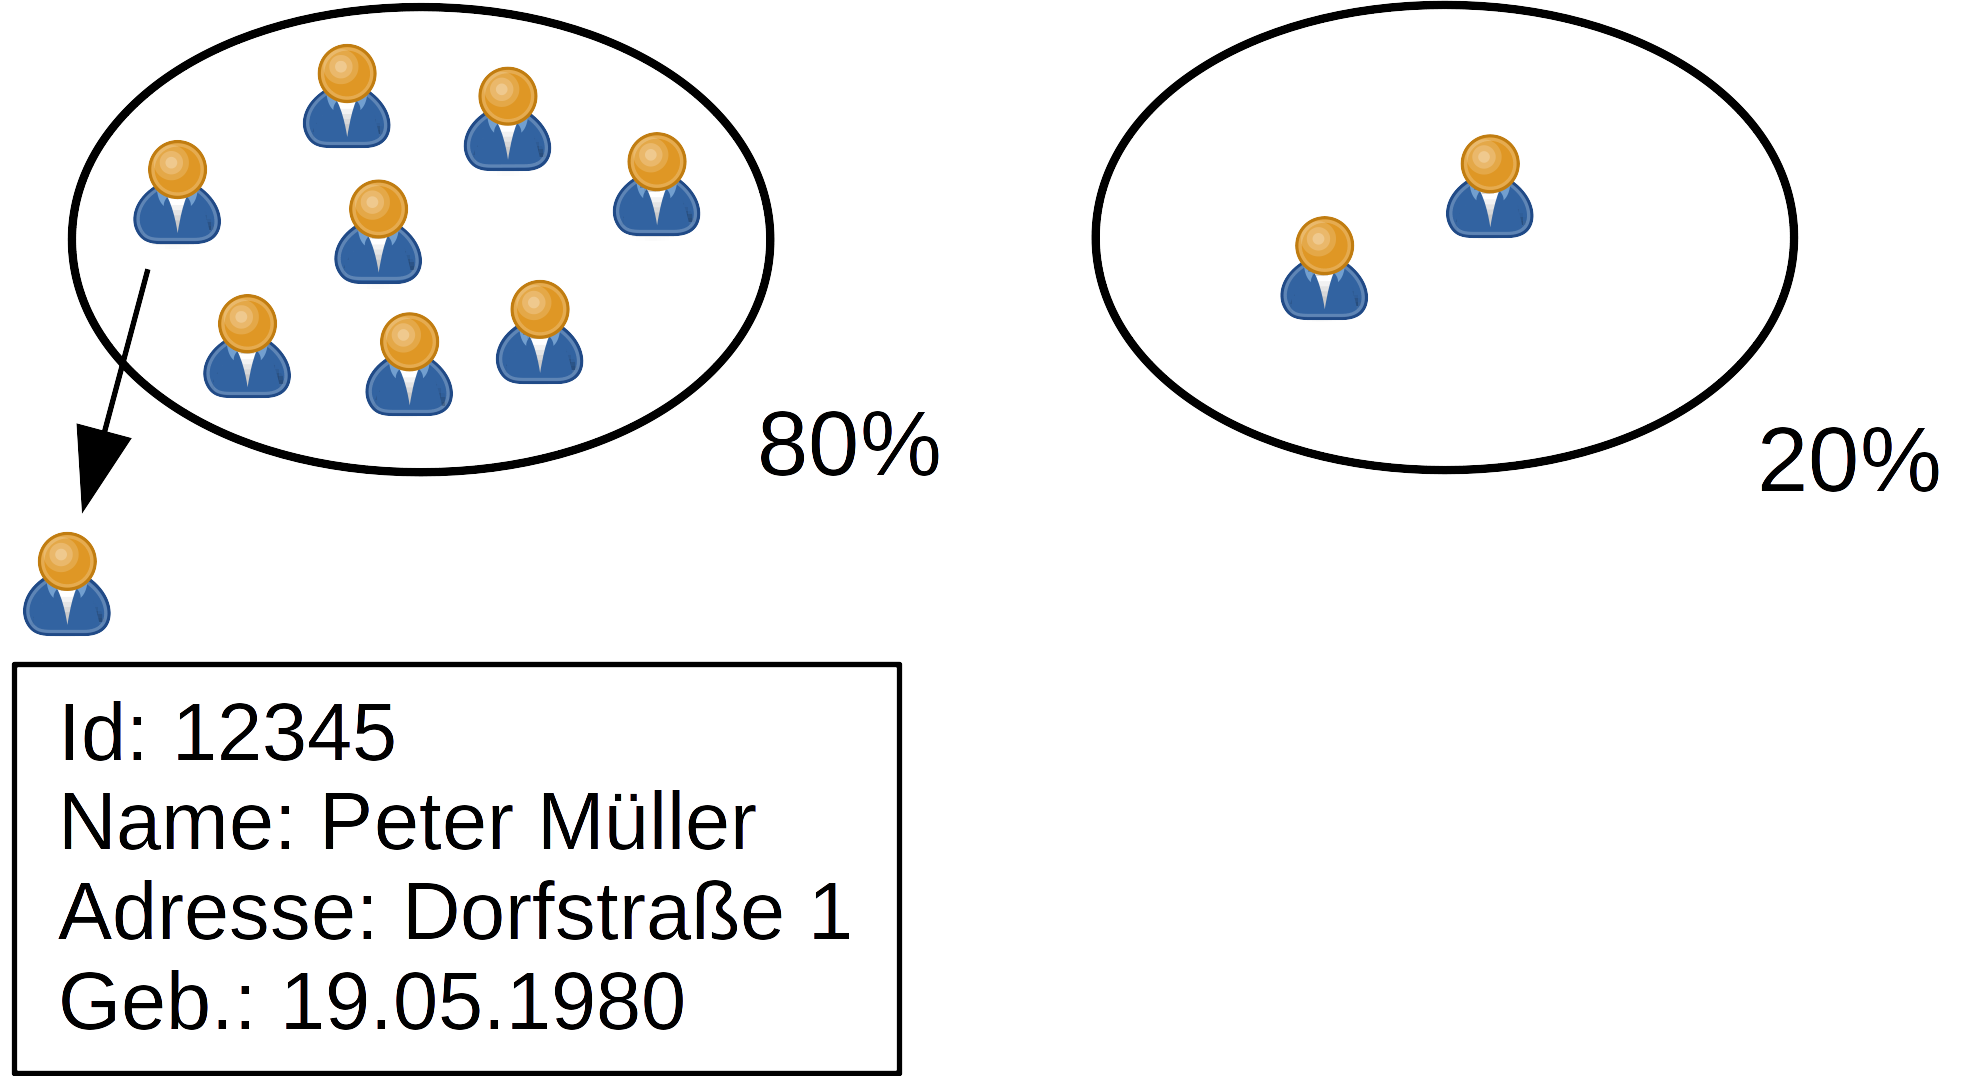
\includegraphics[width=0.5\textwidth]{Bilder/Eingabe.png}};
		\node (start) at (5.5, 3.2) {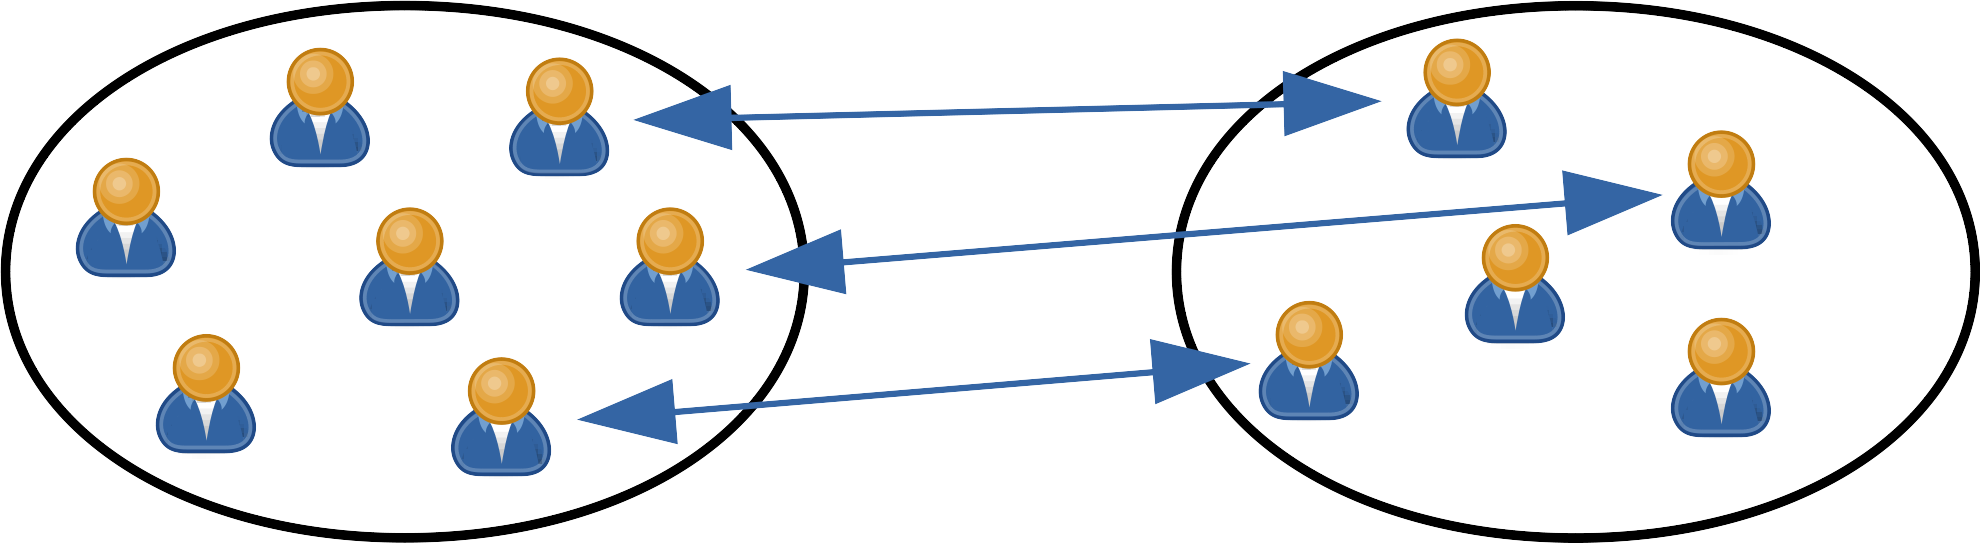
\includegraphics[width=0.5\textwidth]{Bilder/Problem.png}};
	\end{tikzpicture}
\end{frame}

\begin{frame}
	\frametitle{Framework zur Entity-Resolution}

	\begin{itemize}
		\setlength\itemsep{\stdItemSep}
		\item vollständig Parametrisierbar
		\item Modular
		\item Start der Entity-Resolution mit:
		\begin{itemize}
			\setlength\itemsep{\stdItemSep}
			\vspace*{\stdItemSep}
			\item Transformation: Person $\rightarrow$ $V$
			\item Ähnlichkeit: $V \times V$ $\rightarrow$ $[0,1]$
			\item $n$ (Größe der $n$-Gramme)
			\item Threshold
			\item \ldots
		\end{itemize}
		\item sequentieller Nested-Loop
		\begin{itemize}
			\setlength\itemsep{\stdItemSep}
			\vspace*{\stdItemSep}
			\item Vollständige Berechnung der Ähnlichkeit für kartesisches Produkt
		\end{itemize}
	\end{itemize}
\end{frame}


\begin{frame}
	\frametitle{Importphase}
	\begin{center}
	\vspace*{-.2cm}
	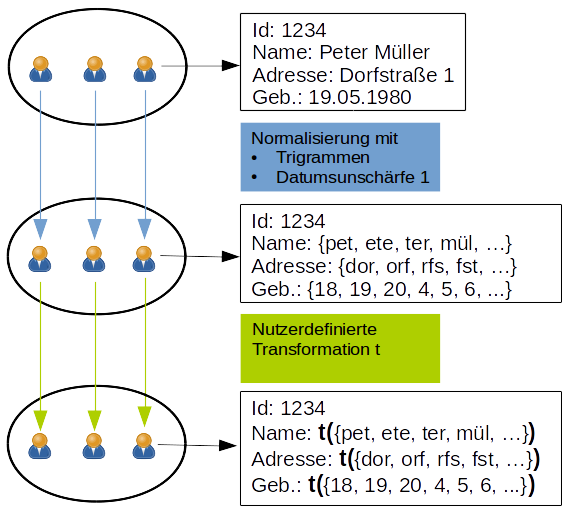
\includegraphics[height=0.9\textheight]{Bilder/Importphase.png}
	\end{center}
\end{frame}
